\section{Pistepilvien käsittelyssä käytetyt tietorakenteet}\label{kirjallisuus}

Tässä luvussa selvitetään, mitä haasteita pistepilvien käsittely asettaa tietorakenteille ja visualisointialgoritmeille. Lisäksi tutustutaan haasteisiin vastaaviin hierarkisista tietorakenteista kirjoitettuihin julkaisuihin.

\subsection{Pistepilvien käsittelyn haasteet}

Suurin haaste pistepilvien käsittelyssä on niiden koko. Nykyaikainen laserkeilain, kuten luvussa \ref{laserkeilaimet} esitetty Leica Geosystemsin RTC360, tuottaa pistepilven, jossa on satoja miljoonia pisteitä. Kun tällaisella keilaimella tehdään useita keilauksia, on pisteiden määrä valtava. Oletetaan esimerkiksi, että suuressa projektissa käytetään pistepilviä, joissa on yhteensä miljardi pistettä. Kun koordinaatit tallennetaan kolmella nelitavuisella liukuluvuulla ja värit RGB-muodossa kolmella tavulla ja lisätään perään vielä yksi täytetavu, voidaan yksi pilven piste esittää 16:lla tavulla. Miljardin pisteen pilvi olisi siis kooltaan 16 gigatavua, joka saattaisi vielä mahtua tehokkaan työaseman keskusmuistiin, mutta ei grafiikkaprosessorin muistiin. Yleensä koko pilveä ei haluta pitää kerralla keskusmuistissa, vaan pisteitä haetaan levyltä muistiin ulkoisen muistin algoritmeilla \engl{out-of-core algorithm}.

Pisteiden määrän vuoksi ei ole realistista olettaa, että kaikki pisteet voitaisiin visualisoida reaaliajassa. Pisteiden määrää voidaan karsia harventamalla pilveä esimerkiksi jakamalla pilvi säännöllisiin kuutioihin, niin sanottuihin vokseleihin, \engl{volume element, voxel}, ja näyttämällä vain yksi piste kustakin vokselista. %TODO: saisko tästä lisää?
Pilven harventaminen kuitenkin aiheuttaa yksityiskohtien katoamista pilvestä, joten sitä täytyy käyttää sovelluskohteesta riippuen maltillisesti. 

Usein on hyväksyttävä, ettei pistepilveä saada visualisoitua reaaliajassa. Interaktiivisessa ohjelmistossa on tärkeää kuitenkin pitää ruudunpäivitystaajuus tarpeeksi korkeana. Tällöin voidaan pistepilvestä piirtää ruudulle ensin karkea yleiskuva, jota tarkennetaan vähitellen, ellei käyttäjä keskeytä visualisointia esimerkiksi vaihtamalla kuvakulmaa. Tällainen astettainen visualisointi on mahdollista käyttämällä hierarkisia tietorakenteita pistepilven käsittelyssä. Tämän tekniikan etuna on se, että käyttäjä näkee välittömästi pistepilven yleisen muodon ilman, että hänen täytyy odottaa, että koko pilvi on visualisoitu. Jos käyttäjällä riittää kärsivällisyys, näkee hän kaikki pilven yksityiskohdat, kun visualisointialgoritmi on käynyt koko tietorakenteen läpi. 


\subsection{Hierarkiset tietorakenteet}\label{tietorakenteet}

Pistepilvien käsittely on paljon tutkittu aihe ja siihen käytetyistä tietorakenteista löytyy paljon julkaisuja. Esitellään seuraavaksi muutama kiinnostava hierarkinen tietorakenne. Aihealueen pioneerityönä pidetään Rusinkiewiczin ja Levoyn Qsplatia, joka onkin antanut vaikutteita uudemmille tietorakenteille. Dachsbacher et al. esittelivät peräkkäispistepuut, jotka voidaan visualisoida hyvin nopeasti grafiikkaprosessorilla. Viime vuosina pistepilvien visualisoinnin tutkimuksen kirkkainta kärkeä on edustanut Wienin teknillisen yliopiston tietokonegrafiikan tutkimusyksikkö. Tämän tutkielman päälähteinä käytetään Claus Scheiblauerin ja Markus Schützin julkaisuja sisäkkäispistepuista.

\subtitle{Qsplat}
Yksi ensimmäisistä pistedatan visualisointiin käytetyistä hierarkisista tietorakenteista on Rusinkiewiczin ja Levoyn esittämä QSplat, joka on kehitetty polygoniverkon visualisointiin pisteiden avulla. Tietorakenne muodostetaan kolmioidusta mallista, jossa kolmioiden normaalit tunnetaan, joten se ei suoraan sovellu raa'an pistepilvidatan käsittelyyn.\footnote{Itse asiassa Rusinkiewicz ja Levoy käyttivät laserkeilatusta pistepilvestä muodostettua kolmioverkkoa, jonka tietorakenne esitti yksinkertaistettuna pistedatana.} QSplatissa on käytetty kuitenkin monia kiinnostavia tekniikoita, joita voi hyödyntää pistepilvien käsittelyssä. \cite{qsplat}

QSplat perustuu puurakenteeseen, jonka solmuissa on avaruutta rajaavia palloja \engl{bounding sphere}. Pallot jakavat avaruutta rekursiivisesti pienempiin osiin siten, että juuren pallo sisältää kaikki kolmiot ja jokainen sisäinen solmu jakaa avaruuden keskimäärin neljään osaan. Puun latva saavutetaan, kun avaruuden jakamisen seurauksena jäljelle jää yksi kolmio. Siitä muodostetaan lehtisolmu, jonka rajaava pallo sisältää koko kolmion. Puun visualisointi onnistuu piirtämällä jokaisen pallon kohdalle sopivan kokoinen täplä \engl{splat}. Puurakenne mahdollistaa myös tehokkaan pisteiden karsimisen. Jos solmun pallo ei ole näkökentässä, eivät sen lapsetkaan ole ja haaraa ei tarvitse käydä läpi. \cite{qsplat}

Puurakenne tallennetaan levylle leveysjärjestyksessä \engl{breadth-first}. Tämän ansiosta puun tasot muodostavat luonnolliset tarkkuustasot \engl{level-of-detail, LOD}: juurisolmun pallo esittää koko mallia, ensimmäinen taso sisältää muutaman pienemmän pallon, ja niin edelleen. Kun tällainen tiedoston sisäinen rakenne yhdistetään ulkoisen muistin tekniikoihin, voidaan täplien piirtäminen aloittaa heti, kun tarpeeksi puun solmuja on ladattu levyltä muistiin.\footnote{Rusinkiewicz ja Levoy päättävät ruudulle projisoitujen täplien koon perusteella kuinka syvälle puussa tulee edetä.} Puun rakennetta on havainnollistettu kuvassa \ref{tarkkuustasot}. \cite{qsplat}

\begin{figure}
    \centering
    %https://tex.stackexchange.com/questions/332300/draw-lines-on-top-of-tikz-forest
    \begin{forest}
        for tree={circle,draw,fill=white,align=center},
    %    my label/.style={
    %        label={[anchor=south,font=\scriptsize,red]:#1},
    %      },
        before drawing tree={
        tikz+={
            \node [anchor=mid east, font=\sffamily] (m) at (current bounding box.west |- .mid) {};
        },
        tempcounta'=-1,
        for tree={
            if={% if the current level exceeds the value of tempcounta
            >OR>{level}{tempcounta}%
            }{% then step the count and add the level marker
            tempcounta'+=1,
            tikz+/.process={ Rw {tempcounta} {
                \node [anchor=mid east, font=\sffamily] at (m.east |- .mid) {taso #1};
                }%
            },
            }{},
        },
        },
        [$a$,name=a
            [$b$,name=b
                [$d$,name=d
                    [$h$,name=h]
                    [,phantom]
                ]
                [$e$,name=e
                    [$i$,name=i]
                    [$j$,name=j]
                ]
            ]
            [$c$,name=c
                [$f$,name=f
                    [,phantom]
                    [$k$,name=k]
                ]
                [$g$,name=g
                    [,phantom]
                    [,phantom]
                ]
            ]
        ]
        \draw[->,dotted,thick,relative,red] (a) to[out=-20,in=200] (b);
        \draw[->,dotted,thick,relative,red] (b) to[out=0,in=180] (c);
        \draw[->,dotted,thick,relative,red] (c) to[out=20,in=290] (d);
        \draw[->,dotted,thick,relative,red] (d) to[out=0,in=180] (e);
        \draw[->,dotted,thick,relative,red] (e) to[out=0,in=180] (f);
        \draw[->,dotted,thick,relative,red] (f) to[out=0,in=180] (g);
        \draw[->,dotted,thick,relative,red] (g) to[out=30,in=300] (h);
        \draw[->,dotted,thick,relative,red] (h) to[out=0,in=180] (i);
        \draw[->,dotted,thick,relative,red] (i) to[out=0,in=180] (j);
        \draw[->,dotted,thick,relative,red] (j) to[out=0,in=180] (k);
        %\begin{scope}[->,dashed,thick,blue]
        %  \draw ([shift={(-0.1,0.1)}]a.north west) -- ([shift={(-0.1,0.1)}]b.north west);
        %  \draw ([shift={(-0.1,0.1)}]b.north west) -- ([shift={(-0.1,0.1)}]d.north west);
        %\end{scope}
    \end{forest}
    \caption{Puun läpikäyntijärjestys (punainen katkoviiva) muodostaa luonnolliset tarkkuustasot}
    \label{tarkkuustasot}
\end{figure}

Toinen hyödyllinen QSplatissa käytetty tekniikka on koordinaattien kvantisointi \engl{quantization}. Kun tarkkuudesta voidaan tinkiä, solmujen pallojen absoluuttisia koordinaatteja ei tallenneta, vaan niiden sijainti ilmaistaan suhteessa vanhempiinsa. Pallon säteen ja keskipisteen suhteellisen poikkeaman ilmaisemiseen käytetään vain 13:a arvoa. Pallon säde $r$ voi olla välillä $[\frac{1}{13}, \frac{13}{13}]$ ja samaten keskipisteen suhteellisen poikkeaman $x, y$ ja $z$ -koordinaatit ovat vanhemman pallon läpimitan kolmastoistaosan monikertoja. Kun vielä hylätään vanhemman pallon ulkopuolella olevat keskipisteet ja käytetään hakutaulua, voidaan pallon sijainti esittää vain 13:lla bitillä, kun normaali liukulukuesitys vaatisi vähintään 16 tavua. \cite{qsplat}

QSplat onnistui visualisoimaan 1,5-2,5 miljoonaa pistettä sekunnissa, mikä on sen aikaisella laitteistolla erinomainen tulos \cite{qsplat}. Kuten sanottu, se ei sellaisenaan kuitenkaan sovellu laserkeilattujen pistepilvien käsittelyyn. Pistepilvien pisteiden normaaleja ei yleensä tiedetä, joten ne pitäisi esiprosessointivaiheessa selvittää esimerkiksi luvussa \ref{workflow} esitetyllä tekniikalla. QSplat tarjoaa kuitenkin monia tekniikoita, joita pistepilviä käsittelevässä tietorakenteessa voidaan hyödyntää, kuten hierarknen rakenne ja koordinaattien suhteellinen esitystapa.
%Toisena ongelmana voidaan pitää tapaa, jolla mallin kolmioita esitetään palloina. Tietorakenteeseen luodaan nimittäin uutta dataa, kun lehtisolmuihin tallennettujen, yhden kolmion sisältävien pallojen lisäksi ylemmillä tasoilla on keinotekoisia, monia kolmioita kuvaavia palloja.



\subtitle{Peräkkäispistepuut}
Dachsbacher et al. esittelevät niin kutstutun peräkkäispistepuun \engl{sequential point tree}, jossa pisteet on aluksi järjestetty samaan tapaan pallopuuhun kuin QSplatissa. Pisteet sijaitsevat puun lehtisolmuissa ja sisäsolmuissa säilytetään täpliä, jotka juuri ja juuri peittävät solmun lasten rajaavat pallot. Täplien väri määräytyy lapsisolmujen värien keskiarvolla. \cite{spt}

Jokaiseen puun solmuun on virhelaskelmien perusteella lisätty rajat katseluetäisyydelle, jolla solmu valitaan visualisoitavaksi. Visualisointivaiheessa hierarkia litistetään taulukoksi, joka voidaan syöttää suoraan grafiikkaprosessorille. Grafiikkaprosessori käy taulukkoa läpi ja valikoi sopivat solmut, joiden perusteella täpliä piirretään ruudulle. \cite{spt}

Peräkkäispistepuut voidaan visualisoida nopeasti grafiikkaprosessorin käytön ansiosta, mutta niissä on myös heikkouksia. Tietorakenteen vaatimuksena on, että kaikki data mahtuu grafiikkaprosessorin muistiin. Näin on vain pienillä malleilla ja tilannetta pahentaa se, että peräkkäispistepuut eivät ole kovin säästäväisiä muistin suhteen. Hierarkian jokaisessa sisäsolmussa luodaan lisää dataa, kun lapsisolmujen unionia kuvataan täplän sijainnilla ja koolla, sekä keskimääräisellä värillä.

Wimmer ja Scheiblauer esittävät parannuksia peräkkäispistepuihin. Uusien täplien luomisen sijaan puun sisäsolmuissa valitaan lapsisolmuista edustaja, joka parhaiten kuvaa sisäsolmun esittämää avaruuden osaa. Tämä on tärkeä huomio, sillä käsiteltäessä massiivisia pistepilviä tulisi välttää ylimääräisen datan luomista. Hierarkiasta muodostetaan tarkkuustasot siten, että alemmat tarkkuustasot sisältyvät ylempiin tasoihin ja visualisoitaessa oikea tarkkuustaso valitaan täplien koon ja katseluetäisyyden perusteella. Solmua vastaavan täplän koko määräytyy siitä, kuinka syvällä hierarkiassa se on. Wimmer ja Scheiblauer kutsuvat tätä rakennetta muistioptimoiduksi peräkkäispistepuuksi. \engl{memory optimized sequential point tree, MOSPT} \cite{ip} %Kun hierarkian läpikäymistä jatketaan niin pitkälle, että solmujen täplät ovat yhden pikselin kokoisia, ei lopputulokseen jää aukkoja. \cite{ip}


\subtitle{Sisäkkäispistepuut}
Wimmer ja Scheiblauer kritisoivat muistioptimoituja peräkkäispistepuita siitä, että ne eivät tue näkökentän ulkopuolisten pisteiden tehokasta karsimista ja siitä, ettei muistioptimointi yksinään riittänyt poistamaan tarvetta ulkoisen muistin algoritmeille. Ratkaisuksi he esittivät sisäkkäisiä oktettipuita \engl{nested octree}. Oktettipuu\footnote{Tätä suomennosta on käyttää esimerkiksi \cite{oktettipuu}} on yksinkertainen avaruutta rekursiivisesti jakava tietorakenne, jonka jokainen sisäsolmu jakaa kuvaamansa avaruuden osan kahdeksaan osaan. Wimmerin ja Scheiblauerin tietorakenteessa oktettipuita on kahdessa tasossa. Ulompaa oktettipuuta käytetään avaruuden jakamiseen, sen tehokkaseen läpikäymiseen ja näkökentän ulkopuolisten alueiden karsimiseen. Ulomman puun jokainen solmu sisältää yhden sisemmän oktettipuun, joka vastaa samaa avaruuden osaa, kuin ulkoisen puun solmu. Pisteet sijoitetaan sisempiin puihin, yksi jokaiseen solmuun. \cite{ip}

\begin{figure}
    \centering
    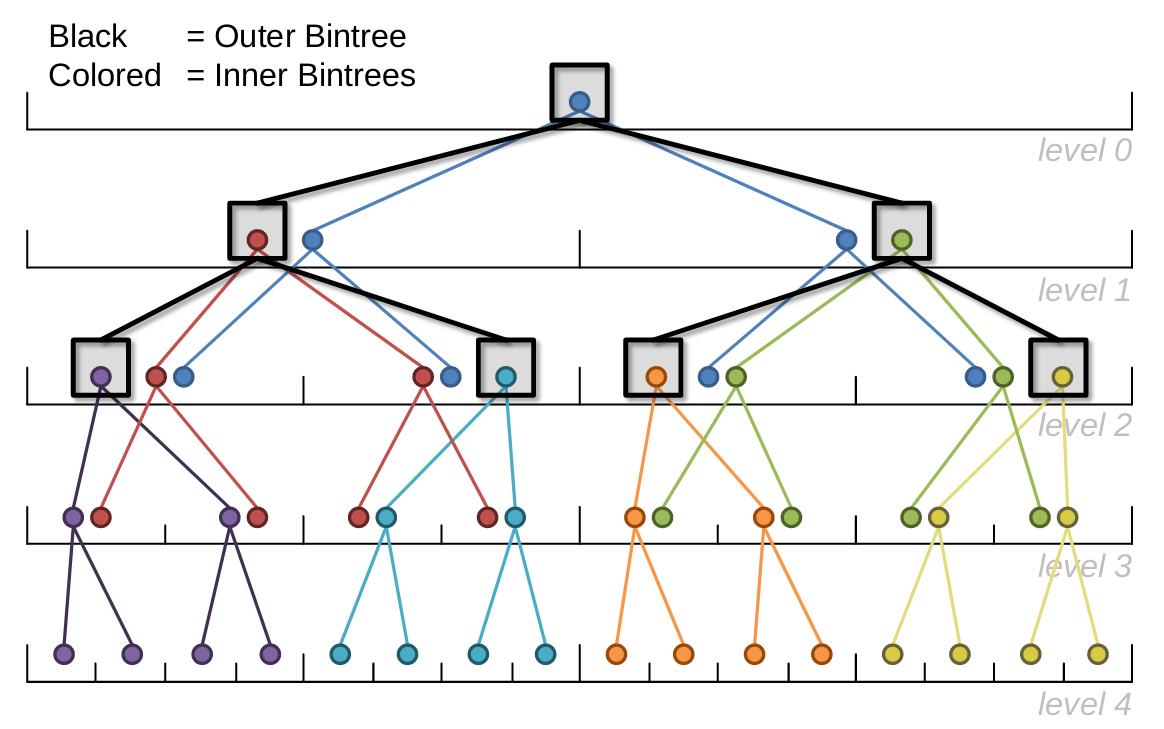
\includegraphics[width=0.6\paperwidth]{img/nested.png}
    \label{nested}
    \caption{Sisäkkäinen binääripuu, jossa sekä ulomman, että sisempien puiden syvyys on kolme. Ulompaa puuta kuvaavat mustat neliöt ja sisempää värikkäät ympyrät. Puista muodostuu viisi tarkkuustasoa. Kuva: \cite{scheiblauer}}
\end{figure}

Sisäkkäisistä oktettipuista luodaan tarkkuustasot siten, että sisemmistä puista kerätään pisteitä ulomman puun tasojen mukaan. Tarkkuustasoon kuuluvat pisteet sijaitsevat siis ulomman puun samalla tasolla, mutta useiden sisempien puiden eri tasoilla. Tarkkuustasojen muodostumista on havainnollistettu kuvassa \ref{nested}. Puut tallennetaan levylle tarkkuustaso kerrallaan, mikä mahdollistaa ulkoisen muistin algoritmien käytön. Visualisoitaessa tarvitsee levyltä lukea pisteitä vain haluttuun tarkkuustasoon asti, eikä loppuja pisteitä tarvitse ladata muistiin. \cite{ip}

Scheiblauer jalostaa sisäkkäisten oktettipuiden ideaa väitöskirjassaan esittelemällä muokattavat sisäkkäiset oktettipuut \engl{modifiable nested octree, MNO}. Jos edellä esiteltyjä sisäkkäisiä oktettipuita halutaan muokata rakentamisen jälkeen, on sisemmät puut rakennettava ja muokattu hierarkia tallennettava levylle uudestaan. Nimensä mukaisesti MNO mahdollistaa tehokkaan pisteiden lisäämisen ja poistamisen. \cite{scheiblauer}  

MNO:n rakenne eroaa sisäkkäisistä oktettipuista siten, että sisemmät puut korvataan säännöllisillä, kolmiulotteisilla ruudukoilla, joihin pisteet tallennetaan. MNO:n rakentaminen alkaa juurisolmusta, joka vastaa kaikki pisteet peittävää avaruutta. Solmun sisältämä ruudukko jakaa solmua kuvaavan avaruuden osan $128^3 = 2 097 152$ soluun. Pisteitä lisätään puuhun yksi kerrallaan niin, että jokaiseen ruudukon soluun mahtuu vain yksi piste. Jos solu on varattu, sijoitetaan piste ylimääräiseen taulukkoon odottamaan, että vastaavia pisteitä kertyy tarpeeksi, jotta olisi järkevää luoda uusia solmuja puuhun. Kun ennaltamäärätty vähimmäismäärä pisteitä on kertynyt ylimääräisten pisteiden taulukkoon, luodaan ruudukon sisältävälle solulle lapsisolmuja ja sijoitetaan ylimääräiset pisteet niihin. Ruudukkoon sijoitettavien pisteiden määrälle on hyvä asettaa myös yläraja. \cite{scheiblauer}

Jokainen tietorakenteen solmu tallennetaan omaan tiedostoonsa levylle, josta niitä ladataan muistiin visualisointivaiheessa tarvittaessa. Visualisointialgoritmiin kuuluu käyttäjän asettama pistebudjetti, joka asettaa ylärajan yhdessä ruudunpäivityksessä piirrettävien pisteiden määrälle.\footnote{Scheiblauer testasi pistepilvivisualisoijaansa asettamalla rajan vain sataantuhanteen pisteeseen.} Tätä rajaa säätämällä käyttäjä saa jonkinlaisen kontrollin ruudunpäivitystaajuuden suhteen. \cite{scheiblauer}

Tiedostorakenne mahdollistaa hierarkian yksinkertaisen muokkaamisen. Lisättäessä uusia pisteitä MNO:hon tarkastetaan ensin, sijoittuuko se juurisolmun kuvaamaan avaruuden osaan. Jos näin on, onnistuu lisääminen kuten rakennusvaiheessa. Muussa tapauksessa juurisolmulle luodaan vanhempia kunnes jokin niistä muodostaa tarvittavan kokoisen avaruuden, ja piste lisätään sen ruudukkoon. Kun puun vanhan juuren yläpuolelle luodaan uusia solmuja, jää niiden ruudukot vajaaksi. Tällöin alemmista solmuista nostetaan pisteitä ylöspäin niin kauan, kunnes vajaita ruudukoita on vain lehtisolmuissa. Pisteiden poistaminen puusta on triviaalia, kun sisäsolmuihin mahdollisesti jäävät tyhjät ruudukot täytetään kuten pisteitä lisättäessä. \cite{scheiblauer}


Markus Schütz jatkoi Wimmerin ja Scheiblauerin työtä esittelemällä opinnäytetyössään verkkoselaimessa ajettavan Potree-nimisen pistepilvivisualisoijan. Potreen käyttämä tietorakenne perustuu Scheiblauerin muokattaviin sisäkkäisiin oktettipuihin, mutta hierarkian rakennusvaiheessa kiinnitetään huomiota pisteiden tasaiseen jakautumiseen solmujen välille. Oktettipuun sisäsolmujen ruudukoihin hyväksytään uusia pisteitä vain, jos ne ovat tarpeeksi kaukana muista ruudukon pisteistä. Lehtisolmut hyväksyvät ennaltamäärättyyn rajaan saakka kaikki pisteet, kunnes ne muutetaan sisäsolmuiksi ja liian lähekkäin olevat pisteet jaetaan uusien lapsisolmujen kesken. \cite{potree}

Potree käyttää ulkoista muistia tehokkaasti ja pystyy käsittelemään jopa 640 miljardia pistettä sisältäviä pistepilviä.\footnote{Kyseinen pistepilvi (Actueel Hoogtebestand Nederland, ANH2, \url{http://ahn2.pointclouds.nl/}) kuvaa koko Alankomaiden valtiota ja se vaatii 7,68 teratavua tallennustilaa. Potreen tietorakenteessa pistepilvi jakautui 13:lle tasolle ja 38:aan miljoonaan solmuun.} Rakennusvaiheessa oktettipuun solmuja tallennetaan tasaisin väliajoin levylle, jottei muisti täyttyisi. Kun jokainen solmu tallennetaan omaan tiedostoonsa, on yksittäisten solmujen tallentaminen ja lukeminen levyltä helppoa. Massiivisia pistepilviä kuvaavat hierarkiatkin voivat olla satojen megatavujen kokoisia. Schütz ratkaisee suurten hierarkioiden nopean lataamisen verkon yli jakamalla senkin puurakenteeseen. Näin voidaan välttää sekä turhien pisteiden, että näkökentän ulkopuolella olevien hierarkian haarojen lataaminen muistiin. \cite{potree}

Potreen visualisointialgoritmi priorisoi niitä hierarkian solmuja, jotka ovat lähellä katselupistettä ja joiden kuvaruudulle projisoitu koko on suurin. Visualisoinnin suorituskykyä voidaan säädellä Scheiblauerin toteutuksen mukaisesti käyttäjän asettamalla pistebudjetilla. Schütz on kehittänyt Potreehen myös hienostuneen, grafiikkaprosessorilla ajettavan algoritmin mukautuvaan pisteiden koon määrittämiseen; pistepilven harvemmissa osissa piirretään pisteet suurempina, jottei reikiä esiintyisi. \cite{potree}